\section{Worksheet 9}
\begin{lstlisting}
bool AreaLight::sample(const float3& pos, float3& dir, float3& L) const
{	
	const IndexedFaceSet& normals = mesh->normals;
	int n_faces = mesh->geometry.no_faces();
	
	uint3 random_triangle = mesh->geometry.face(rand() % n_faces);
	float xi_1 = mt_random();
	float xi_2 = mt_random();
	
	float u = 1 - sqrt(xi_1);
	float v = (1 - xi_2) * sqrt(xi_1);
	float w = xi_2 * sqrt(xi_1);
	
	float3 light_pos = u * mesh->geometry.vertex(random_triangle.x) + v * mesh->geometry.vertex(random_triangle.y) + w * mesh->geometry.vertex(random_triangle.z);
	//light_pos = mesh->compute_bbox().center();
	
	dir = light_pos - pos;
	float dir_norm = length(dir);
	dir = normalize(dir);
	
	float3 intensity = make_float3(0.0f);
	for (int i = 0; i < n_faces; i++) {
		uint3 face = mesh->geometry.face(i);
		float3 face_normal = normalize(normals.vertex(face.x) + normals.vertex(face.y) + normals.vertex(face.z));
		intensity = intensity + dot(-dir, face_normal) * get_emission(i) * mesh->face_areas[i];
	}
	
	float epsilon = 1e-4;
	float cutoff_distance = dir_norm - epsilon;
	Ray shadow_ray = Ray(pos, dir, 0, epsilon, dir_norm-epsilon);
	HitInfo hit_info = HitInfo();
	tracer->trace_to_any(shadow_ray, hit_info);
	
	if (!hit_info.has_hit) {
		L = intensity / (dir_norm * dir_norm);
	}
	return !hit_info.has_hit;
	
}
\end{lstlisting}

\begin{figure}[H]
	\centering
	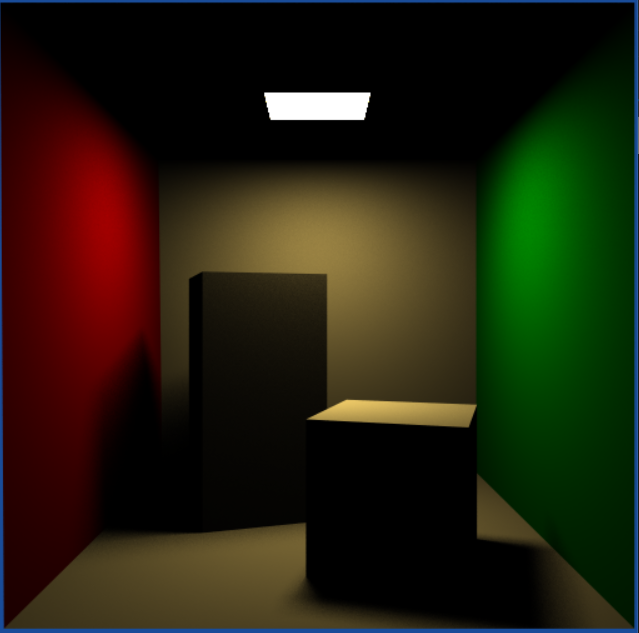
\includegraphics[scale=\imagescale]{images/worksheet_9/soft_shadow}
	\caption{Cornell box with soft shadows}
	\label{fig:cornell_soft_shadows}
\end{figure}

\begin{lstlisting}
float3 Holdout::shade(const Ray& r, HitInfo& hit, bool emit) const
{
	float ambient = 0.0f;
	for (int i = 0; i < samples; i++) {
		float3 dir = sample_cosine_weighted(hit.shading_normal);
		Ray new_ray = Ray(hit.position, dir, 0, 1e-4, RT_DEFAULT_MAX);
		HitInfo new_hit;
		tracer->trace_to_closest(new_ray,new_hit);
		if (!new_hit.has_hit)
		ambient = ambient + 1;
	}
	
	return ambient*tracer->get_background(r.direction);
}
\end{lstlisting}

\begin{figure}[H]
	\centering
	\subfloat[\centering Without holdout plane]{{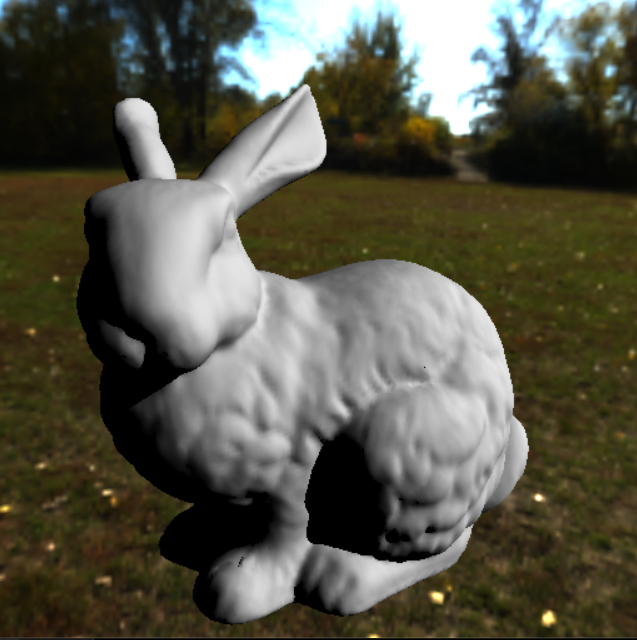
\includegraphics[width=5cm]{images/worksheet_9/bunny_no_holdout} }}%
	\qquad
	\subfloat[\centering With holdout plane]{{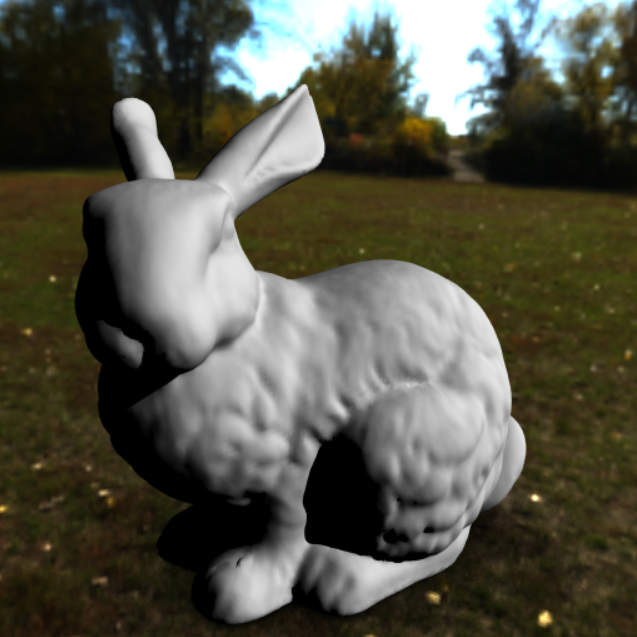
\includegraphics[width=5cm]{images/worksheet_9/bunny_soft_shadow} }}%
	
	\caption{Comparison of renderings of a bunny with and without an holdout plane}%
	\label{fig:holdout_comparison}%
\end{figure}

\begin{figure}[H]
	\centering
	\subfloat[\centering Without holdout plane]{{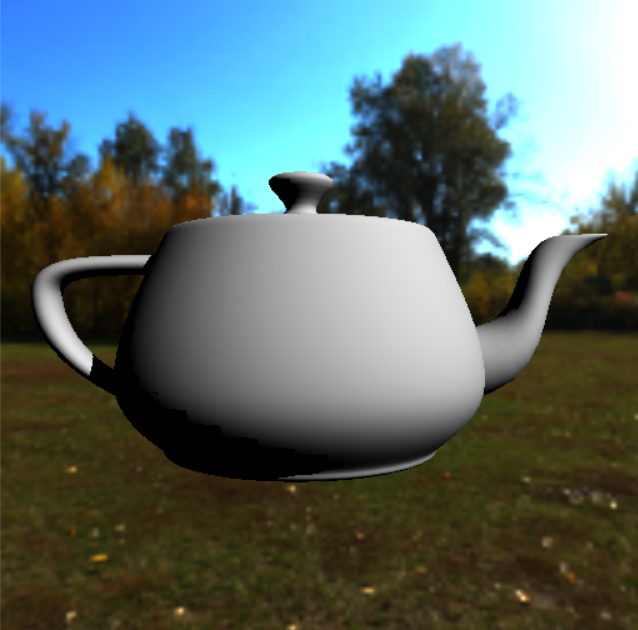
\includegraphics[width=5cm]{images/worksheet_9/teapot_no_holdout} }}%
	\qquad
	\subfloat[\centering With holdout plane]{{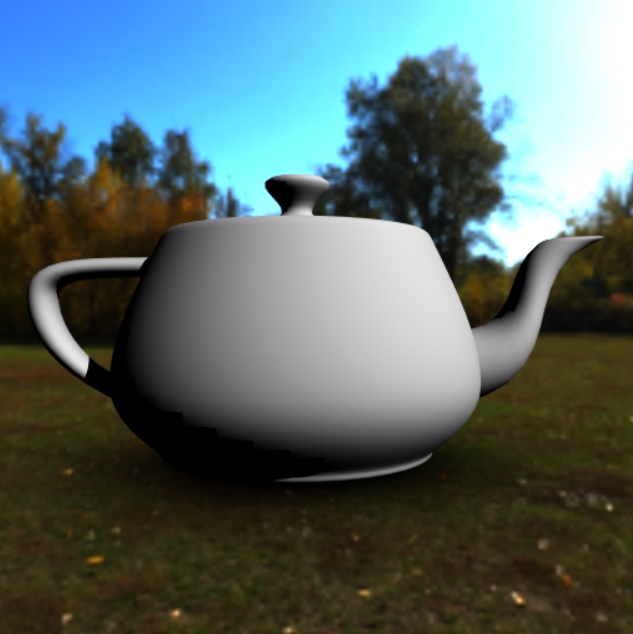
\includegraphics[width=5cm]{images/worksheet_9/teapot_soft_shadow} }}%
	
	\caption{Comparison of renderings of a teapot with and without an holdout plane}%
	\label{fig:holdout_comparison}%
\end{figure}